\documentclass[11pt,aspectratio=169]{beamer}
\usetheme{CambridgeUS}
\beamertemplatenavigationsymbolsempty
\usepackage{fontspec}
\setsansfont{Junicode}
\usepackage{amsmath,mathtools}
\usepackage{hyperref}
\usepackage{graphicx}
\usepackage{xpatch}
\usepackage[export]{adjustbox}
\usepackage{pgfplots}
\usepackage{tikz}
\usetikzlibrary{shapes,calc,matrix,decorations.markings,decorations.pathreplacing,positioning, intersections,backgrounds,through,hobby}
\usepackage{csquotes}
\usepackage[french]{babel}
\date[2 octobre 2023]{2 octobre 2023}
\author[Matthias \textsc{Gille Levenson}]{\\~\\ Matthias \textsc{Gille Levenson}\\   {\scriptsize AMU -- CIHAM UMR 5648}\\ {\tiny prénom [point] gille [point] levenson [at] ens-lyon.fr}\vspace{-1cm}}
\title[Transcription automatisée et HTR]{Rappels sur XPath}
\titlegraphic{\includegraphics[scale=0.23]{/home/mgl/Bureau/Travail/admin/logos/logo-ciham.png}}


%\usepackage[labelformat=empty]{caption}
\setbeamertemplate{caption}{\insertcaption\par}

\usepackage[datamodel=thesis,citestyle=authoryear,isbn=true,
doi=true,backend=biber,language=french,url=true,sorting=nty,maxnames=6, maxcitenames=4]{biblatex}
\renewbibmacro{in:}{}
\renewcommand*{\bibfont}{\tiny} 
% http://mcclinews.free.fr/latex/introbeamer/elements_contenu.html
%\xapptobibmacro{cite}{\setunit{\nametitledelim}\printfield{year}}{}{}
\addbibresource{biblio.bib}

\begin{filecontents*}{thesis.dbx}
\ProvidesFile{thesis.dbx}[2014/06/14 supervisor for theses]
\RequireBiber[3]
\DeclareDatamodelFields[type=list,datatype=name]{supervisor}
\DeclareDatamodelEntryfields[thesis]{supervisor}
\end{filecontents*}


\begin{filecontents*}{french-thesis.lbx}
\ProvidesFile{french-thesis.lbx}[2014/06/14 english for thesis]
\InheritBibliographyExtras{french}
\NewBibliographyString{supervision,jointsupervision}
\DeclareBibliographyStrings{%
inherit           = {french},
supervision       = {{dirigée par}{dir\adddotspace }},
jointsupervision  = {{codirigée par}{codir\adddotspace }},
}
\end{filecontents*}

\DeclareLanguageMapping{french}{french-thesis}

\newbibmacro*{thesissupervisor}{%
  \ifnameundef{supervisor}{}{%
    \ifnumgreater{\value{supervisor}}{1}
      {\bibstring{jointsupervision}}
      {\bibstring{supervision}}
    \printnames{supervisor}}}

\xpatchbibdriver{thesis}
  {\printfield{type}}
  {\printfield{type}
   \newunit
   \usebibmacro{thesissupervisor}}
  {\typeout{yep}}
  {\typeout{no}}
  
% https://tex.stackexchange.com/a/184878 ajout direction thèse





\AtBeginSection[]
{\begin{frame}
 \frametitle{}  
 \tableofcontents[currentsection,
                  hideothersubsections,
                  subsubsectionstyle=show/show/show/hide
                   ]
 \end{frame} 
 }



\setbeamertemplate{sections/subsections in toc}[square]
\setbeamertemplate{bibliography item}[sqare]
\setbeamertemplate{itemize item}[square]
\setbeamertemplate{enumerate item}[square]
\setbeamertemplate{itemize subitem}[square]





\renewcommand*{\dotFFN}{}
\newcommand{\astfootnote}[1]{%
\let\oldthefootnote=\thefootnote%
\setcounter{footnote}{0}%
\renewcommand{\thefootnote}{\fnsymbol{footnote}}%
\footnote{#1}%
\let\thefootnote=\oldthefootnote%
}








\begin{document}
\maketitle



\begin{frame}{Espaces de noms et préfixes}
\begin{itemize}
\item 
\end{itemize}
\end{frame}

\begin{frame}{Le document XML comme un arbre}
\begin{itemize}
\item Le document XML est un arbre qui contient un noeud racine et un certain nombre d'embranchements.
\item On passe d'un niveau à l'autre à l'autre de la barre oblique / comme pour n'importe quel système arborescent comme le système de fichiers: \texttt{~/Bureau/Travail/Cours\_et\_formations/Biblissima-\_scripts\_mss/XPath/diapos} représente un système fonctionnant de la même manière que \texttt{TEI/body/div/div/head}.
\end{itemize}
\end{frame}


\begin{frame}{Application à Andromaque}
\begin{figure}
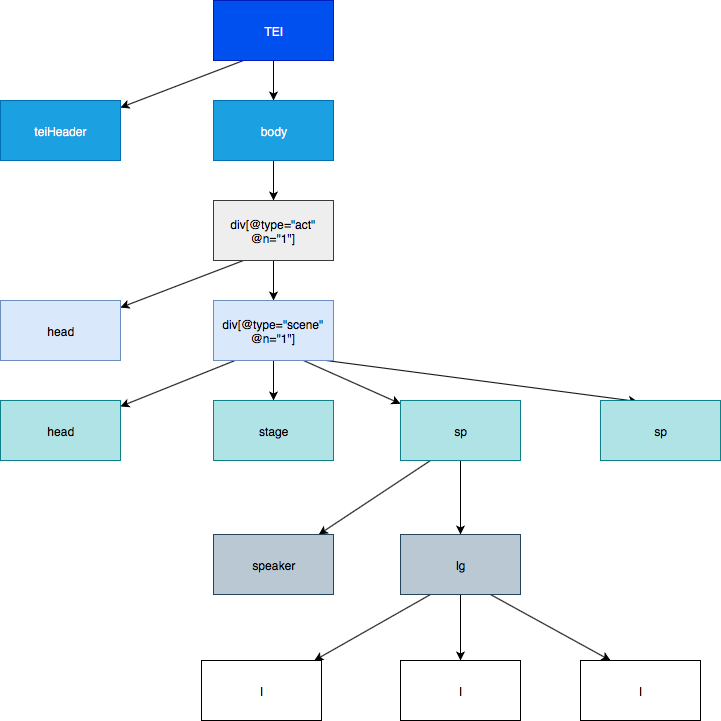
\includegraphics[width=.4\textwidth]{img/andromaque.png}
\end{figure}
\end{frame}

\begin{frame}{Exercice 1}
% Reprendre https://github.com/gabays/Cours_COSME_2019/blob/master/Xpath_FondamentauxXSLT/Xpath_FondamentauxXSLT.md
\begin{itemize}
\item Quels éléments sont sélectionnés par les chemins suivants ?
\begin{itemize}
\item \texttt{TEI/body/div/div};
\item \texttt{TEI/body/div/div/head};
\item \texttt{TEI/body/div/div/sp}.
\end{itemize}
\end{itemize}
\end{frame}

\begin{frame}{Les axes XPath}
\begin{itemize}
\item On peut vouloir naviguer dans l'arbre sans connaître exactement sa structure. Pour ce faire, on aura besoin de naviguer selon les grandes relations entre noeud
\item Un noeud a en effet 0 ou 1 parent, et il peut avoir 0 ou plus enfants. Il peut avoir des ancêtres et des descendants, ainsi que des \enquote{adelphes} (\textit{siblings}).
\item Les \textbf{axes} XPath permettent de représenter ces relations et aident à la navigation dans l'arbre
\item On utilise un axe de la façon suivante (\texttt{axe::noeud}). Ici, le double deux-points est fondamental, il permet de distinguer l'axe du préfixe de l'espace de nommage.
\end{itemize}
\end{frame}

\begin{frame}{Les axes XPath: navigation sur parent proche}
\begin{itemize}
\item \texttt{child}: l'enfant
\item \texttt{parent}: le parent
\item \texttt{preceding-sibling}: l'adelphe précédent (premier enfant précédent du parent)
\item \texttt{following-sibling}: l'adelphe suivant (premier enfant suivant du parent)
\end{itemize}
\end{frame}

\begin{frame}{Les axes XPath: navigation sur parent éloigné}
\begin{itemize}
\item \texttt{ancestor}: n'importe quel noeud ancêtre
\item \texttt{descendant}: n'importe quel noeud descendant
\item \texttt{preceding}: n'importe quel noeud précédant le noeud actuel
\item \texttt{following}: n'importe quel noeud suivant le noeud actuel
\end{itemize}
\end{frame}








\begin{frame}{Expressions conditionnelles ou prédicats}
\begin{itemize}
\item On peut vouloir cibler des noeuds précis et avoir besoin d'exprimer des conditions pour ce faire. Le \textbf{prédicats} permettent d'exprimer ces conditions. Un prédicat se matérialise sous la forme d'une expression entre crochets droits \texttt{[condition]}
\item Cette condition peut être de n'importe quelle forme: il suffit qu'elle soit vraie pour que le noeud soit retourné.
\item On peut ainsi tester l'existence ou l'absence d'un attribut, la valeur d'un attribut, une égalité ou inégalité, comparer des valeurs...
\item Ainsi, dans la transcription diplomatique d'un manuscrit, \texttt{//tei:text/descendant::tei:lb[@break='no']} permettra de sélectionner tous les débuts de ligne qui coupent un mot, soit toutes les coupures de mot à la ligne.
\end{itemize}
\end{frame}



\begin{frame}{Exercice 2}
% Reprendre https://github.com/gabays/Cours_COSME_2019/blob/master/Xpath_FondamentauxXSLT/Xpath_FondamentauxXSLT.md
\begin{itemize}
\item À partir de l’arbre XML simplifié d’Andromaque donner les chemins suivants en partant de l’élément racine TEI
\begin{itemize}
\item Donner le chemin vers \texttt{body};
\item Donner le chemin vers la \texttt{div} dont l'attribut \texttt{@type} est égal à \texttt{act};
\item Donner le chemin vers \texttt{stage};
\item Donner le chemin vers \texttt{speaker};
\item Donner le chemin vers les \texttt{l}.
\end{itemize}
\end{itemize}
\end{frame}



\begin{frame}{Fonctions basiques: \texttt{translate}}
Un certain nombre de fonctions pré-établies sont particulièrement utiles ici. \textbf{Ce sont des fonctions XPath}: vous verrez avec Ariane d'autres fonctions propres à XSLT, et avec Jean-Paul des fonctions propres à XQuery.
\begin{itemize}
\item \texttt{translate(text, str, repl)} produit un \textit{mapping} pour remplacer \textbf{un à un} les éléments de \texttt{str} par les éléments de \texttt{repl} dans le texte donné. 
\item Exemple: \texttt{translate('Longtemps, je me suis couché de bonne heure', 'aeiou', 'uoiea')} produira \enquote{Lengtomps, jo mo sais ceaché do benno hoaro.}
\end{itemize}
\end{frame}

\begin{frame}{Fonctions basiques: \texttt{replace}}
\begin{itemize}
\item \texttt{replace(text, str, repl)} remplace par \texttt{repl} toutes les chaînes \texttt{str} trouvées dans \texttt{text}.
\item Exemple: \texttt{translate('Longtemps, je me suis couché de bonne heure', 'couché', 'endormi')} produira \enquote{Longtemps, je me suis endormi de bonne heure.}
\end{itemize}
\end{frame}


\begin{frame}{Fonctions basiques: type des noeuds visés}
\begin{itemize}
\item Noeuds textuels: \texttt{text()}
\item Noeuds XML: \texttt{element()}
\item Commentaires: \texttt{comment()}
\item Noeud en général: \texttt{node()}
\end{itemize}
\end{frame}

\begin{frame}{Fonctions basiques: modifier la casse (XPath 2.0)}
\begin{itemize}
\item \texttt{lower-case(text)}
\item \texttt{upper-case(text)}
\end{itemize}
\end{frame}


\begin{frame}{Fonctions basiques: identifier des sous-chaînes de caractères}
\begin{itemize}
\item \texttt{substring-before(text, string)}
\item \texttt{substring-after(text, string)}
\end{itemize}
\end{frame}


\begin{frame}{Fonctions basiques: manipuler des chaînes de caractères multiples }
\begin{itemize}
\item \texttt{concat(text1, text2, text3, ..., textN)}: concatène l'ensemble des chaînes de caractères indiquées par l'utilisateur.ice. Les arguments ne peuvent être que des éléments textuels uniques et non pas des séquences
\item \texttt{string-join(chemin)}: concatène l'ensemble du texte trouvé dans le chemin. (XPath 2.0)
\end{itemize}
\end{frame}


\begin{frame}{Fonctions basiques: \texttt{compter}}
\begin{itemize}
\item \texttt{count(path)}
\end{itemize}
\end{frame}

\begin{frame}{Fonctions basiques: la position}
\begin{itemize}
\item Tous les noeuds ont une position, \textbf{qui commence à 1}. Elle peut être décidée à l'aide d'un prédicat et de la fonction \texttt{position()}: \texttt{//library/bookshelfA/book[position() = 3]} ou plus simplement \texttt{//library/bookshelfA/book[3]}
\item La position est déterminée par rapport à l'expression XPath qu'elle suit.
\item On peut récupérer le dernier élément d'une liste avec la fonction \texttt{last()}
\end{itemize}
\end{frame}


\begin{frame}{Exercice 3}
Nous allons travailler avec le sonnet 17 de Shakeaspeare, présent dans le répertoire \texttt{XPath} du dépôt. On travaille sur Oxygen.
\begin{itemize}
\item Trouvez tous les vers dont le schéma métrique correspond au schéma canonique du sonnet.
\item Trouvez tous les vers qui présentent une divergence par rapport au schéma métrique canonique du sonnet
\item Comptez le nombre de césures dans le sonnet
\item Identifiez le vers qui comprend la deuxième césure
\item Identifiez le texte du vers qui vient après la première césure
\end{itemize}
\end{frame}

%\begin{frame}
%\frametitle{Plan} % Table of contents slide, comment this block out to remove it
%\tableofcontents % Throughout your presentation, if you choose to use \section{} and \subsection{} commands, these will automatically be printed on this slide as an overview of your presentation
%\end{frame}



%\begin{frame}[allowframebreaks]{Références}
%\printbibliography[keyword=dataset, title={Jeux de données}]
%\hrule
%\printbibliography[notkeyword=dataset, title={Sources secondaires}]
%\end{frame}

\end{document}
